\section{Durchführung}
\label{sec:Durchführung}
Der Versuch wird wie in der Abbildung \ref{fig:Aufbau} aufgebaut.
\begin{figure}
    \centering
    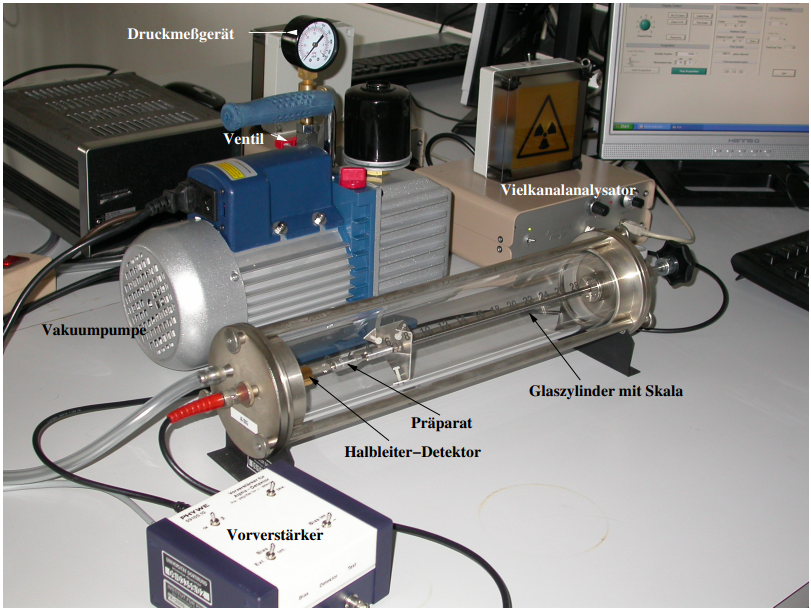
\includegraphics[scale=0.5]{content/Aufbau 701.png}
    \caption{Versuchsaufbau.}
    \label{fig:Aufbau}
\end{figure}
Bei dem Präparat handelt es sich um ein Am-Präparat. Der Vielkanalanalysator ist mit dem Computer verbunden.
Im Programm MCA wird der Schalter auf connectet gestellt.\\


\noindent Zur Messung der Reichweite und Energieverlust der $\alpha$-Strahlung wird die Messzeit auf $\qty{120}{s}$ gestellt.
